\chapter{Transparent Healthcare}

\section{Information seeking}

% Growing quantity of information available
The quantity of cancer information available in the media and on the internet has been growing rapidly over the past decades. While it is getting easier to find health related materials online, the vast quantity of resources makes it harder to assess the entirety of the information \cite{viswanath_science_2005,viswanath_communications_2012}.

% Cancer information is important
After being diagnosed with cancer, patients and family members are expected to make difficult treatment choices that might have serious, life-long consequences. Such decisions require some understanding of the complexity of the disease as well as the treatment. It is a situation fraught with stress and uncertainty, but a time when information might help. At the time of diagnosis and during the course of treatment and post-treatment, most patients and family members are eager to have information on the status or the stage of disease, different treatment options, clinical trials, and alternative and complementary therapies \cite{butow_dynamics_1997,cassileth_information_1980}.

% Patients want information
Today, understanding is growing about the importance of involving cancer patients in decision-making about their care, with the literature identifying an association between participation in decision-making by patients and their families and improved patient satisfaction and quality of life \cite{sheabudgell_information_2014}.

63.7\% of the online population in the US looked for health information for themselves or others at least once in the previous 12 months. Despite newly available communication channels, physicians remained the most highly trusted information source to patients. Although more patients are looking for information online before talking with their physicians \cite{hesse_trust_2005}.

% How do patients get their information ?
The most frequently reported source of information was the Internet \(57.4\%\); other commonly used sources of information included a health provider \(32.6\%\), brochures or pamphlets \(25.1\%\), and cancer organizations \(24.3\%\). The most frequently reported types of information sought included information about a specific type of cancer \(43.1\%\), treatment or cures for cancer \(29.4\%\), prognosis or recovery from cancer \(29.0\%\), and prevention of cancer \(27.0\%\). The least frequently reported types of cancer information sought included where to get medical care \(3.4\%\), paying for medical care or insurance \(4.6\%\), and cancer organizations \(5.4\%\).

% Patients are not always satisfied with the amount of information they receive
There is increasing evidence to suggest that patients with cancer require more information about their disease and its consequences than they receive \cite{mcpherson_effective_2001}.

During treatment, they might seek information on coping with side effects and symptom management. The exchange of information between healthcare providers and patients, however, does not always lead to satisfaction; it could also lead to misunderstanding, and patients might even forget parts of the discussions \cite{ley_communicating_1988,hogbin_getting_1989}.

Several participants shared stories about not receiving the most up-to-date cancer information. Cancer survivors and caregivers learned about the latest cancer treatments and were able to access the best available research. Participants shared stories of diagnostic failures in which symptoms had been undiagnosed, incorrectly diagnosed, or dismissed by their healthcare provider. Survivors presenting with rare cancers or unusual side effects encountered healthcare providers with a lack of clinical expertise in treating their disease and, consequently, turned to the Internet. Survivors required practical information to help them manage their illness at home and found help from their online communities. Participants exercised power through direct confrontation with their healthcare providers, which included behaviors such as questioning, persuasion, and coercion. Armed with the ``right questions to ask'' survivors and caregivers challenged healthcare providers. Participants influenced their care and treatment plan by exerting persuasive power in their relationship with healthcare providers. The limitations of self-selection sampling bias inherent in survey research and the lack of socio-demographic data are outweighed by the established trustworthiness of the current study and the richness of the data set \cite{dolce_internet_2011}.

The increased usage of the Internet by cancer patients thus puts new demands on health care professionals. Patients need advice about how to find reliable and credible web sites and also help with authenticating and interpreting the information they find \cite{carlsson_cancer_2009}.

% Benefits of having information
Carefully designed communication interventions have an impact on the patient's knowledge and recall, patient satisfaction and their ability to manage the symptoms \cite{johnson_effects_1982,hack_feasibility_1999,mohide_randomised_1996,mcpherson_effective_2001}. Some evidence indicates that preparing patients ahead of time for the clinical visit by providing practical information has a beneficial effect \cite{huchcroft_testing_1984,cegala_patient_2003}.

The demonstrated benefits of information seeking for cancer patients, coupled with increases in information availability, underscore the importance of monitoring patient information seeking experiences over time \cite{finney_rutten_cancer-related_2016}.

Communication facilitates the patients involvement in their own healthcare, reduces distress, improves adherence to, and compliance with, treatment regimens and increases the patient's sense of control \cite{viswanath_science_2005}.

Considerable research shows that medically related education interventions are most effective when they are tailored to patients' individual needs. While this matter is relevant to all patient communication skills training, it may be especially relevant to cancer patients \cite{cegala_patient_2003}.

% Impact of the lack of information
Newly diagnosed breast cancer patients who need health information but experience difficulties in accessing it may be at risk for experiencing poorer psychosocial health \cite{arora_barriers_2002}.

% Disparities in information accessibility
Developments in ICTs offer an unprecedented opportunity to overcome the conventional barriers of place, class, and race. It is conceivable that information on cancer risk can be communicated with a greater degree of specificity and customization to different audiences, which may minimize inequalities. Additionally, ICTs have the potential to leverage the resources that exist among patients, caregivers, and the general public so that social support and other resources are more easily shared. At the same time, patients and caregivers may be better informed and better able to engage in participatory models of care \cite{viswanath_communications_2012}.

Unfortunately, the deployment of ICTs, a 21st century phenomenon, is taking place in the context of classic 20th Century divides of class, place, and race—and they seem to exacerbate these divides instead of abating them \cite{viswanath_race_2011}.

A lower likelihood of cancer information seeking was also observed among those with lower education levels and those with incomes below \$20,000. Controlling for socio-demographic factors, a lower likelihood of cancer information seeking was observed among those aged 75 and older. This finding is of particular concern given the greater likelihood of developing cancer with age \cite{finney_rutten_cancer-related_2016}.


\section{Quality of care}

\section{Healthcare-Network web application}

\begin{figure}[H]
    \includegraphics[width=0.7\textwidth]{images/healthcare-network/home.png}
    \centering
    \caption{
        \textbf{Healthcare-Network: homepage.} A minimalist page with a search bar allowing to find hospitals based on their name, category, or location.
    }
    \label{fig:hn-home}
\end{figure}


\begin{figure}[H]
    \includegraphics[width=0.7\textwidth]{images/healthcare-network/search.png}
    \centering
    \caption{
        \textbf{Healthcare-Network: search results.} The list of retrieved hospitals and their details is displayed, as their position on a map. This query shows all the \ac{chru} hospitals in metropolitan France.
    }
    \label{fig:hn-search}
\end{figure}


\begin{figure}[H]
    \includegraphics[width=0.7\textwidth]{images/healthcare-network/curie-services.png}
    \centering
    \caption{
        \textbf{Healthcare-Network: description of health services offered, and statistics on \ac{mco} activity for Institut Curie Paris hospital.}
    }
    \label{fig:hn-curie-services}
\end{figure}


\begin{figure}[H]
    \includegraphics[width=0.7\textwidth]{images/healthcare-network/curie-cancero.png}
    \centering
    \caption{
        \textbf{Healthcare-Network: description of oncology activity for Institut Curie Paris hospital.}
    }
    \label{fig:hn-curie-cancero}
\end{figure}


\begin{figure}[H]
    \includegraphics[width=0.7\textwidth]{images/healthcare-network/curie-dp.png}
    \centering
    \caption{
        \textbf{Healthcare-Network: number of patients per cancer related diagnosis for Institut Curie Paris hospital.} Comparison with the median statistics from hospitals within the same category (\ac{clcc}) and overall median.
    }
    \label{fig:hn-curie-dp}
\end{figure}


\begin{figure}[H]
    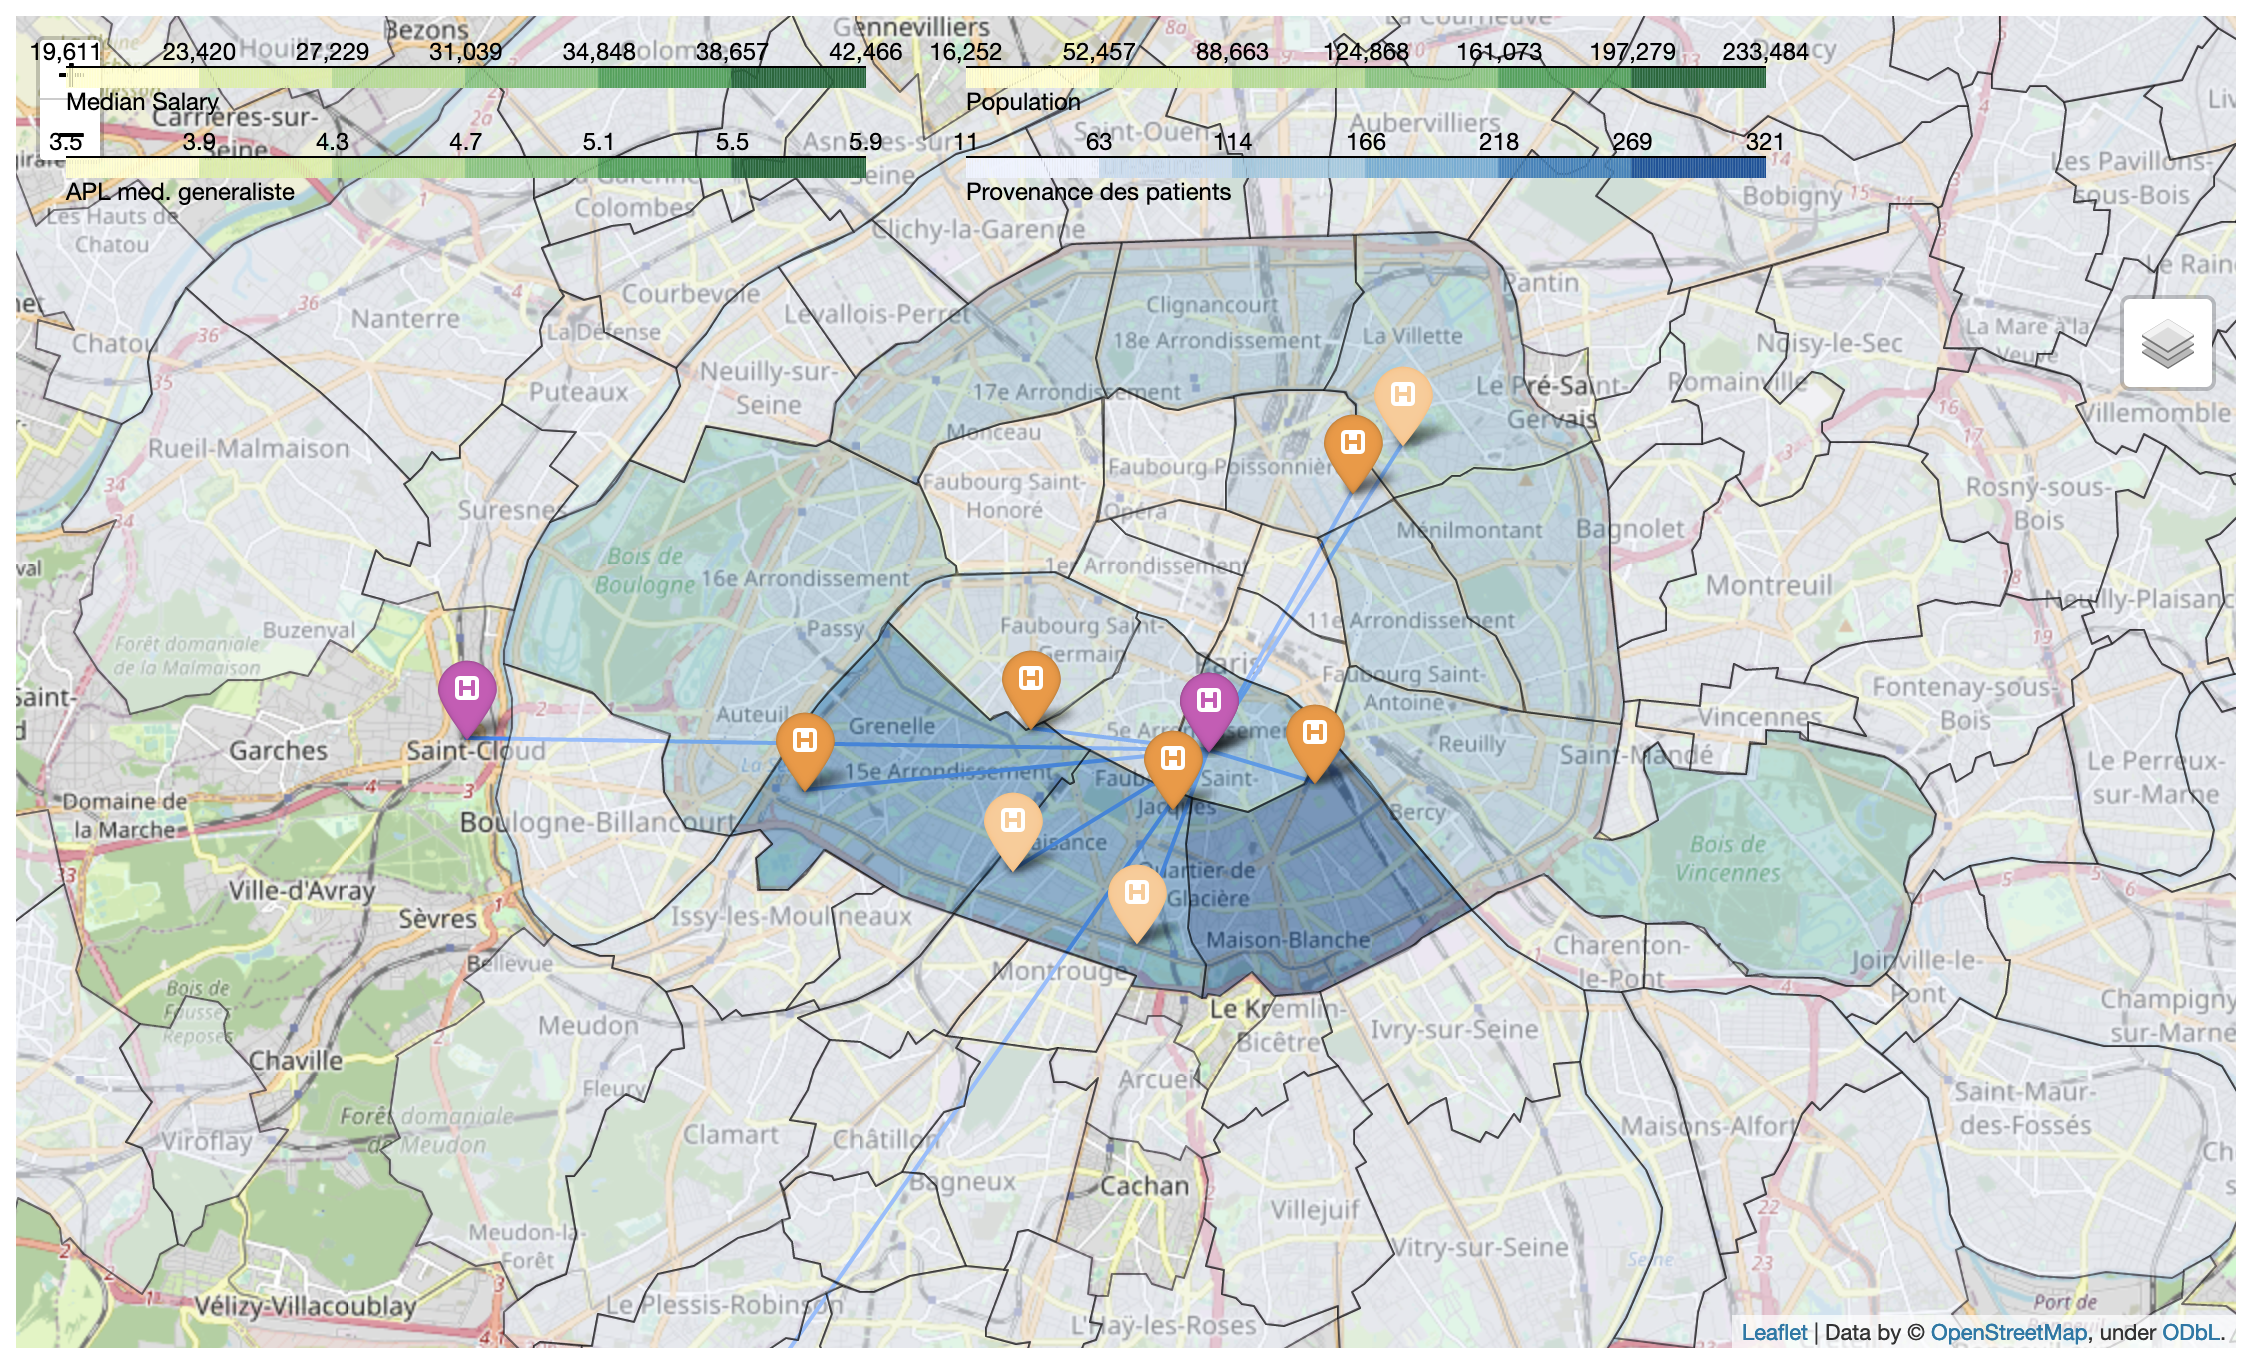
\includegraphics[width=0.7\textwidth]{images/healthcare-network/curie-co-occ.png}
    \centering
    \caption{
        \textbf{Healthcare-Network: map of the hospitals that have the most co-occurrences with Institut Curie Paris.} Co-occurrences between two hospitals are defined as the number of patients who visited both hospitals during their care pathways. To illustrate facility attractiveness, municipalities are colored by the number of inhabitants who visited the Institut Curie Paris hospital.
    }
    \label{fig:hn-curie-co-occ}
\end{figure}


\begin{figure}[H]
    \includegraphics[width=0.7\textwidth]{images/healthcare-network/curie-commune.png}
    \centering
    \caption{
        \textbf{Healthcare-Network: statistics on the municipality where Institut Curie Paris is located (Paris 75105).} Population, median salary and accessibility to primary care are displayed to qualify the hospital neighborhood. Health professionals within the department are also listed to illustrate the health supply available around the hospital.
    }
    \label{fig:hn-curie-commune}
\end{figure}
